% NOTE TO AIP TYPSETERS: TO CONVERT FROM TWO-COL TO PREPRINT, SWITCH
% COMMENTOUT COMMAND FROM A TO B IE. use
% \newcommand{\commentoutA}[1]{}
% \newcommand{\commentoutB}[1]{#1}
% instead of the following
\newcommand{\commentout}[1]{}
\newcommand{\commentoutA}[1]{#1}
\newcommand{\commentoutB}[1]{}
\renewcommand{\thefootnote}{\fnsymbol{footnote}}

\commentoutA{\documentclass[prb,aps,twocolumn,showpacs,twocolumngrid,superbib]{revtex4}}
\commentoutB{\documentclass[prb,aps,nobibnotes,showpacs,superbib,preprint]{revtex4}}

\usepackage{graphicx}
\usepackage{amsfonts}
\usepackage{amsmath}
\usepackage{bm}
\usepackage{alltt}
%\usepackage{epsfig}
%%
%%

\begin{document}

\date{\today}

\title{Linear scaling computation of the Fock matrix VII. Pure \\ 
       Density Functional Theory with periodic boundary conditions}

\author{C.J. Tymczak and Matt Challacombe}

\affiliation{
Theoretical Division, Los Alamos National Laboratory,
Los Alamos, NM 87545, USA}

\begin{abstract}
Periodic boundary conditions have been implemented in the linear scaling
Quantum Chemistry code \textbf{MondoSCF}. For the two-electron Coulomb
matrix, this has been achieved with an exact multipole expansion of
the long range Coulomb field. This yields a spherically summed boundary
condition that is easily transformed to Ewald boundary conditions.
In order to achieve linear scaling of the local Coulomb field, a Quantum
Chemical Tree Code (QCTC) is used. Periodic boundary conditions have
also been incorporated into calculations of the local exchange-correlation
matrix and the exact-exchange matrix. A Hierarchical Cubature (HiCu),
pure Cartesian adaptive grid is used for the local exchange-correlation
matrix. This method achieves linear scaling through the use of advanced
data structures (k-d trees) that maximally exploits locality of the
density. Finally, the current capabilities of MondoSCF for large condensed
phases will be demonstrated.\\[.1cm]
\noindent{\bf Keywords}: self-consistent-field, linear-scaling,tree-code, adaptive numerical integration, Gaussian-orbital
\end{abstract}

\pacs{02.60.Dc,31.15.Ne,71.15Dx,71.15Nc}


\maketitle

\footnotetext[3]{\tt Tymczak@LANL.Gov}
\footnotetext[6]{\tt MChalla@LANL.Gov}
\footnotetext[4]{Preprint LA-UR-03-XXXX.}

\section{INTRODUCTION}
In recent years several successful methods for the calculating the electronic structure of
molecular or condensed matter systems have been developed,
for example Hatree-Fock \cite{slater,CRoothaan51}, Density Functional theory 
\cite{hohen,KohnSham65} or Configuration interaction \cite{Choudhury79}. 
All these methods attempt to solve for the electronic structure via
the many-body quantum problem to within some consistent approximation scheme.
For complex molecular or condensed matter 
system, where chemical reactions are of central importance, these electronic structure
method are essential. Unfortunately, most electronic structure quantum chemistry codes
scale very poorly with system size due to the need to diagonalize the Hamiltonian,
which scales $O(N^3)$ 
%
% Should cite standard comercial code like ``Gaussian''. (Ha)
%
This severely limits the systems sizes 
that these codes can address. Therefore, it has become increasing important for
the development of quantum chemistry codes which scale linearly with increasing 
system size, and several quantum chemistry codes of this type are in 
development 
\cite{Goedecker94,Challacombe96,Canning96,Briggs96,EHernandez96,Scuseria99,ANiklasson02B}. 
However, for reasons of simplicity most of these quantum 
chemistry codes have yet to incorporate periodic boundary conditions.
Unfortunately many
technically important systems can only be addressed within a condensed phase environment,
where surface effects have been removed \cite{Allen90}. Therefore, the inclusion of 
periodic boundary conditions into existing linear scaling quantum chemistry
codes is essential. 

We have implemented periodic boundary conditions into the linear scaling
quantum chemistry code \textbf{MondoSCF} 
\cite{Challacombe96,Challacombe97,Challacombe99}.
For the one electron matrix this has been achieved by a re-summation
over periodic cell images, which because of locality leads to an efficient
calculation of the one electron matrices. For the two electron matrices
various methods are employed. For the two-electron Coulomb matrix,
we achieve this via an exact multi-pole expansion of the long range
Coulomb field \cite{White94,Challacombe97b}. This yields a spherically
summed boundary condition that is easily transformed into the Ewald boundary
condition \cite{Redlack72,Redlack75}. In order to achieve linear
scaling of the local Coulomb field, a Quantum Chemical Tree Code (QCTC)
is used \cite{WarSal93,WarSal95,Salmon:93,Challacombe96A}. For the calculations of the 
local exchange-correlation matrix, a Hierarchical Cubature (HiCu), pure 
Cartesian adaptive grid
is used. This method achieves linear scaling through the use of advanced
data structures (k-d trees) that maximally exploits locality of the
density, and allows for an efficient treatment of the periodic effects
\cite{Bentley79}. All \textbf{MondoSCF} calculations are done at the gamma-point.
This is because the main focus of the \textbf{MondoSCF} linear scaling quantum chemistry
code is large systems, where for insulators k-space integrations become unnecessary 
\cite{Nunes94}.


To demonstrate and validate the capabilities of \textbf{MondoSCF}, we show results for 
three condensed phase systems, Sodium Chloride, Magnesium Oxide 
and Carbon in the diamond structure. We then compare these results to the periodic
Gaussian code \textbf{Crystal98} \cite{Crystal98}. Next we demonstrate that
the code achieves {\it true} linear scaling for the dense periodic diamond system 
up to 512 atoms in the unit cell.
%
% Example system
%
To show the full capabilities of \textbf{MondoSCF} we calculate the surface reconstruction
of the Silicon (111) surface with a step.
%
Finally we give some conclusion concerning the accuracy and utility of \textbf{MondoSCF}
and future research directions.

\commentout{

\section{The Kohn-Sham Equations}

Following the seminary work of Kohn and Sham\cite{KohnSham65}, we start with the KS single 
particle equation
\begin{equation}
H \phi_{i}({\bf r})  = \epsilon_i \phi_{i}({\bf r})
\end{equation}
where the effective Hamiltonian is
\begin{equation}
H = -{\nabla}^{2}+ V_{ext}({\bf r}) + J[\rho({\bf r})] + K_{xc}[\rho({\bf r})]
\end{equation}
and
\begin{equation}
 \rho({\bf r}) = \sum_{i=1}^{N_{el}} | \phi_{i}({\bf r}) |^2
\end{equation}
\begin{equation}
 J[\rho({\bf r})] = \int d{\bf r'} {\rho({\bf r}) \over |{\bf r}-{\bf r'}|},
\end{equation}
and the exchange correlation potential can be calculated from several approximate
functionals
\cite{Becke93,Hertwig97,Bauschlicher95,Adamo00}. In what follows we will 
discuss the calculation of each of the terms in the Hamiltonian 
and how they are calculated in the non-orthogonal Gaussian basis
with the inclusion of periodic boundary conditions.

}


\pagebreak


\section{boundary conditions, linear scaling and notation}

In conventional implementations of periodic boundary conditions, 
Bloch functions 
\begin{equation}
\psi_a({\bf r},{\bf k})  =  \sum_{\bf R} e^{i {\bf k}\cdot {\bf R}} \phi_a ({\bf r}-{\bf R}),
\end{equation}
are often constructed from non-orthogonal functions local to the unit cell (UC). Here, the local function
$\phi_a$ is a Gaussian-Type Atomic Orbital (GTAO) centered on atom {\bf A}, while the 
sum on $\bf R$ runs over the Bravais lattice defined by integer translates of the primitive 
lattice vectors {\bf a}, {\bf b} and {\bf  c}.   These Bloch functions (crystal orbitals)
yeild all possible translational symmetries through variation of the reciprocal lattice vector $\bf k$.     
For small system sizes with high symmetry, a carefull sampling of reciprocal space is required 
for an accurate description of the periodic system.  An alternative approach to including these
important symmetries is to set ${\bf k}=0$ but to use a larger supercell created through replication 
and translation of the primitive UC.  This is the supercell $\Gamma$-point approximation, used
primarily for the study of defects and vacencies rather than as a replacement for $\bf k$-space integration,
perhaps due to the expense of conventional algorithms and slow convergence for small gap systems.

\pagebreak


In this contribution, ${\cal O}(N)$ algorithms are developed specifically for the the $\Gamma$-point 
approximation, allowing the use of large supercells in the case of high symmetry and large primary UCs 
in the case of disordered systems.  While the $\bf k$  dependence is avoided, lattice summation and formal integration over 
the unit cell volume, $V_{\rm UC}$ are retained, at first sight making matrix construction seem quite different than in the 
gas phase,  where integrals are typically taken over all space, $V_\infty$.  Thus, elements of the gas phase overlap matrix 
\begin{equation}
\label{Sab_norm}
S_{ab}=\int _{V_{\infty }}\, d{\mathbf{r}}\, \phi _{a}({\mathbf{r}})\phi _{b}
({\mathbf{r}})
\end{equation}
become 
\begin{equation}
\label{Sab_pbc1}
S_{ab}=\sum _{\mathbf{R},\mathbf{R}'}\int _{V_{\rm UC}}\, d{\mathbf{r}}\, 
\phi _{a}({\mathbf{r}+\mathbf{R}})\phi _{b}({\mathbf{r}+\mathbf{R}'})
\end{equation}
in the periodic regime.  
This formalism can be changed via the 
transformation $\sum_{\bf R} \int_{V_{\rm UC}} d {\bf r} f({\bf r+R}) \rightarrow \int_{V_\infty} d {\bf r} f({\bf r})$,
allowing use of conventional analytic integral technologies \cite{twoels}.  With this 
transformation, elements of the periodic overlap matrix become
\begin{equation}
\label{Sab_pbc2}
S_{ab}=\sum _{\mathbf{R}}\int _{V_{\infty }}\, d{\mathbf{r}}\, \phi _{a}
({\mathbf{r}})\phi _{b}({\mathbf{r}+\mathbf{R}}).
\end{equation}
Under this transformation, it is convienient to define the half summed, intermediate 
basis function products (distributions)
$\rho _{ab}^{\scriptscriptstyle \infty}({\mathbf{r}})=\sum _{\mathbf{R}}\phi _{a}({\mathbf{r}})\phi _{b}
({\mathbf{r}+\mathbf{R}})
$ associated with integration over $V_\infty$.  We likewise denfine an intermediate 
electron density $\rho^{\scriptscriptstyle \infty}({\bf{r}})= \sum _{ab}{\bf{P}}_{ab} \rho _{ab}^{\scriptscriptstyle \infty}({\mathbf{r}})$,
where $\bf P$ is the one-electron reduced density matrix.  
In this convention, elements of periodic overlap matrix become simply 
$S_{ab}=\int  d{\mathbf{r}}\, \rho^{\scriptscriptstyle \infty}_{ab}({\mathbf{r}})$, while the electron count is
$N_{\rm el} =\int  d{\mathbf{r}}\, \rho^{\scriptscriptstyle \infty}({\mathbf{r}})$.


It is worth noting that the complexity of $\rho^{\scriptscriptstyle \infty}$ is ${\cal O}(N)$, due to the
exponential prefactor factor $e^{- \chi_{ab} ({\bf A}-{\bf B}-{\bf R})^2}$ that results from the Gaussian product theorem
and occurs in each term  $\rho^{\scriptscriptstyle \infty}_{ab}$.  Thus, the implicit sum over {\bf A}, {\bf B} and {\bf R} involves $N$-scaling 
non-zero terms, which are easily eliminated {\em a priori}.  For small exponents  $\chi_{ab}$, care must be excersized in 
truncation of periodic sums to avoid overlap matrices that are not positivie definate.  While these situations
can be avoided simply with tighter neglect criteria, they are often due to use of basis sets designed for gas phase 
calculations in conjunction with small UCs.  An alternative is to use one of the Crystal basis sets \cite{} or 
increasing the most diffuse uncontracted exponent(s).

\pagebreak

\section{data structures and error estimates}\label{datastruct}

Both the Quantum Chemical Tree-Code (QCTC) \cite{} for computing the Coulomb matrix and Hierarchical Cubature (HiCu)
for computing the Exchange-Correlation matrix are fast ${\cal O}(N {\rm lg} N)$ algorithms that 
intimately couple underlying data structures and error estimates.  It is important to understand some 
of these particulars first, before addressing their extension to periodic boundary conditions.
Also, the current version of QCTC is quite different from perevious descriptions \cite{}, and deserves some
introduction.  

Both QCTC and HiCu are homeomorphic, involving $k$-d tree representation of the density.  
In our implementations, $k$-d trees are doubly linked lists with an Axis Aligned Bounding Box (AABB) for each node.
This bounding box contains all the spatial information about a node and its children, 
allowing fast ${\cal O}({\rm lg} N)$ look up of overlapping components through AABB intersection tests \cite{}, 
wich have become well developed in the ray tracing litterature \cite{}.
In the case of QCTC, this fast look up constitutes the penetration acceptability criterion (PAC) \cite{}, which identifies
preliminary algomerations of the electron density that may be accurately represented via a multipole 
approximation due to the absense of charge-charge penetration effects.  For accepted aglomerations a second test, 
the multipole acceptability criterion (MAC), is performed to check translation errors in the multipole 
expansion \cite{}.  For each primitive bra distribution, this fast range query is performed on the $k$-d tree 
representation of the total density, leading to a best case partition of near-field and far-field interactions 
in construction of the gas phase Coulomb matrix,
\begin{eqnarray}
J_{ab} &=& \int d {\bf r} \int d {\bf r'} 
\rho_{ab} ({\bf r}) \left|{\bf r}-{\bf r'} \right|^{-1} \rho^{\rm NF}_{\rm tot}({\bf r}) \\
&+&\int d {\bf r} \int d {\bf r'} \rho_{ab} ({\bf r}) \left|{\bf r}-{\bf r'} \right|^{-1} \rho^{\rm FF}_{\rm tot}({\bf r}).
\end{eqnarray}
The QCTC near/far-field partition pushes the multipole approximation to the limit, employing best case error esitmates 
that depend on the extent of the ``bra'' distribution $\rho_{ab}$, and involving tree traversal to the resolution of 
individual distributions.  While resolving individual primitives forgoes well developed technologies for the 
integral evaluation of contracted functions, it allows for the early onset of linear scaling even for dense systems 
such as diamond. 


\newpage
\newpage


In the case of HiCu, two seperate $k$-d tree structures are used.  The rho-tree holds the electron density,
while the cube-tree contains a hierarchical grid for integration of the exchange-correlation potential.  Each node of the 
cube-tree is composed of a Cartesian non-product integration rule with the gridpoints enclosed by it's AABB.
The cube-tree is constructed iteratively through recusrive bisection of the primary volume (the root AABB), using 
exact error bounds to achieve arbitrary precision of the integrated density and its gradients.   As the cube-tree 
is extended, AABB intersection tests are performed while traversing the rho-tree,  avoiding parts of the density 
that do not overlap with that portion of the grid.  Upon construction of the grid,  the inverse procedure is carried out;  
for each primitive distribution, the cube-tree is walked selecting only overlaping portions of the grid via the AABB 
intersection test.


For both of these fast algorithms, the trade off between efficiency and accuracy is controled by the AABB,  which in turn 
depends on the the extent or range $R$ of a primitive Gaussian distribution, $\rho_q$, beyond which it is assumed to 
have negglibible influence.  Of coarse, negglible depends on the use to which the distribution is put, as will become 
obvious in the following. 

Both HiCu and QCTC employ a Hermite Guassian (HG) representation of distributions
\begin{equation}
\rho_q ({\bf r}) = \sum_{lmn} d_{lmn} \Lambda^q_{lmn}({\bf r}),
\end{equation}
where 
\begin{equation}
\Lambda^q_{lmn}({\bf r}) = \frac{\partial^{l+m+n} }{\partial Q^l_x \partial Q^m_y \partial Q^n_z} e^{-\zeta_q ({\bf r}-{\bf Q})^2}.
\end{equation}
which provides an intermediate with elements of the density matrix folded  into the coefficients $d_{lmn}$, and allows
the use of McMurchie-Davidson recurrence relations in analytic integral evaluation.   
A simplification for this form is provided by Cramer's inequality \cite{}, yeilding a 
bound for the behavior of a HG distribution: 
\begin{equation}
\rho_q ({\bf r})  \leq C_q e^{ -\widetilde \zeta_q ({\bf r -Q})^2 },  
\end{equation}
where
\begin{equation}
C_q=\sum_{lmn} \left|d_{lmn}\right| K^3 \left[ 2^{l+m+n} ~ l! m! n! ~ \zeta^{l+m+n}_q \right]^{1/2} ,
\end{equation}
the constant $K=1.09$ and  
\begin{equation}
\widetilde \zeta_q = 
\begin{cases}
\zeta_q   & l+m+n= 0 \\
\frac{1}{2} \zeta_q   & {\rm otherwise.}
\end{cases}
\end{equation}

\newpage
\newpage

In the case of HiCu, the overlap extent $R^{\rm o}_q$ is used, guaranteeing that beyond this range 
numerical evaluation of the distribution $\rho_q$ yeilds an accumulation less than $\tau$;
\begin{equation}
C_q e^{ -\widetilde \zeta_q (R^{\rm o} _q)^2 }  = \tau .
\end{equation}
For QCTC,  errors in the electrostatic potential due to penetration errors must be controlled. 
For this purpose, the penetration extent $R^{\rm p}_q$  found by solving 
\begin{equation}
C_q \int \left[ \left(\pi/{\widetilde \zeta_q} \right)^{3/2} 
\delta({ r})  - e^{ -\widetilde \zeta_q {r}^2 } \right] \left|{ r}-{ R^{\rm p}_q} \right|^{-1} {\rm d} r = \tau ,
\end{equation}
is introduced.  In both HiCu and QCTC, the density-tree is constructed by recursively splitting the largest
box dimension, untill each primitive has been resolved.  Then the primitive AABBs are computed from their
extents and merged recursively up the tree.  For HiCu, this is all there is to it, but for QCTC multipole
moments are also translated to a common center and recursively merged up the tree.  Also, when computing 
matrix elements of $\bf J$, the primitive bra AABB is computed with using $R^{\rm o}_q$, while  $R^{\rm p}_q$ are 
used to construct AABBs of the density-tree.

\newpage
\newpage

\begin{figure}
\resizebox*{3.5in}{!}{\includegraphics{Regions.eps}}\label{regions}
\caption{\label{figure:ReplicateCells} Regions that contribute to $N$-scaling summation of the Coulomb matrix.
The inner cells that make up $V_{\rm in}$ provide a buffer region that gaurantees convergence of the multipole 
expansion of Coulomb interactions between the unit cell and all cells in $V_{\rm PFF}$.  The
periodic far-field region, $V_{\rm PFF}$, is the spherically ordered lattice extending
to infinity but excluding $V_{\rm in}$.  For large cells and high order multipole 
expansions, $V_{\rm in}$ includes just the unit cell and its nearest 27 neigbors, in fast multipole method notation 
corresponding to a well-seperated index of unity.  However, for smaller cells and lower 
order multipole expansions, $V_{\rm in}$ tends to a spherical distribution of cells surrounding the unit cell.   
Direct summation over $V_{\rm PFF}$ leads to charges at the infinite surface  $S_{\infty}$, which must be
be cancelled by tin-foil (conducting) boundary conditions to achieve equivalence with Ewald summation}
\end{figure}

\newpage
\newpage


\section{Periodic Quantum Coulomb Sums}

Under the gamma point approximation, elements of the periodic Coulomb matrix are 
\begin{eqnarray}
J_{ab}&=&\frac{1}{2}\int _{V_{\rm UC}} d{\mathbf{r}}  \int _{V_{\infty }} 
d{\mathbf{r}'}{\rho _{ab}\left( {\mathbf{r}}\right) {\left| \mathbf{r}-\mathbf{r}'\right| }^{-1}
\rho_{\rm tot}\left( \mathbf{r}'\right) } \\
&=& \frac{1}{2}\sum _{\mathbf{R}}\int _{V_{\infty }}\int _{V_{\infty }} 
d{\mathbf{r}}\, d{\mathbf{r}'}{\rho _{ab}^{\scriptscriptstyle \infty}\left( {\mathbf{r}}\right)  
{\left| \mathbf{r}-\mathbf{r}'\right| }^{-1} \rho^{\scriptscriptstyle \infty}_{\rm tot}\left( {\mathbf{r}'}+{\mathbf{R}}\right) }
\nonumber 
\end{eqnarray}
where $rho_{\rm tot}$ is the total, periodic density including both electronic and nuclear terms.  These integrals
involve infinite summation over lattice vectors $\bf R$, and must be handled with care.  There are at least two
main approaches to handling this summation:  Multipole expansion of the Ewald potential \cite{},
or Ewald-like summation of the multipole expansion.    Expansion of the Ewald potential yeilds  
tin foil (TF) boundary conditions, requires reciprocal and real space summation with every $\bf J$ build, 
and scales as $O(N^{3/2})$.  An alternative is the ewald-like summation of the multipole interaction tensor,
which was first described by Nijboer and De Wette (NDW) \cite{} and later reviewd and extended by us \cite{}
to lattice summation of the irregular solid harmonic multipole interaction tensor. 
This Ewald-like summation is taken over the periodic far field, $V_{\rm PFF}$, which is lattice summation excluding 
an inner region, $V_{\rm in}$, surrounding the unit cell that has been subtracted to guarantee convergence of the 
multipole expansion.  Because ${\cal M}^{m}_l$ maybe cheaply precomputed and reused, 
the cost of Coulomb summation over the PFF scales as as ${\cal O}(N p^2)$ ({\bf CJ verify!!}), where $p$ is the order 
of the multipole expansion.  With this feature, achieving $N$-scaling quantum Coulomb sums involves the contributions
\begin{equation}
{\bf J} = {\bf J}^{\rm In} + {\bf J}^{\rm PFF} + {\bf J}^{\rm TF} \, ,
\end{equation}
corresponding to the three seperate regions shown in Fig.~\ref{}.   Here, $J_{\rm In}$ is computed using 
the fast ${\cal O}(N {\rm lg} N)$ QCTC algorithm outlined previously in Section~\ref{datastruct}. Construction of ${\bf J}_{\rm PFF}$ 
will be developed in the following section, while in Section~\ref{} the term ${\bf J}_{\rm TF}$ nessesary to 
introduce tin-foil boundary conditions is detailed.

\newpage
\newpage

\subsection{The Periodic Far Field}

The periodic far field (PFF) term in the Coulomb matrix
\begin{equation}
J_{ab}^{\rm PFF} = \sum _{{\bf R}\in {\rm PFF}} \int \int d {\bf r} d {\bf r'}  \rho^\infty_{ab}({\bf r}) {\left| {\bf r}-{\bf r'}+{\bf R} \right|}^{-1}
\rho^\infty_{\rm tot} ({\bf r'})
\label{PFFOne}
\end{equation}
involves charge distributions that are well seperated with respect to both penetration and the
convergence of multipole expansion errors, as outlined in Fig.~\ref{regions}. 

With these conditions, and assuming the unit cell is centered at the origin, the multipole expansion \cite{} 
\begin{eqnarray}
{| {\bf r}-{\bf r}'+{\bf R}|}^{-1} &\approx&
\sum^p_{l=0} (-1)^{l}  \,
\sum^p_{l'=0} \Bigl[
\\
&&\sum^{l}_{m=-l} \,
\sum^{l'}_{m=-l'} 
O^{m}_{l}({\bf r})
            \,M^{m+m'}_{l+l'}({\bf R})
            \,O^{m'}_{l'}({\bf r}')  \Bigr] , \nonumber
\end{eqnarray}
employing the regular and irregular solid harmonics, $O^l_m$ and $M^l_m$ respectively, 
may be inserted into Eq.~(\ref{PFFOne}) yeilding
\begin{eqnarray}
J_{ab}^{\rm PFF}& =&\sum _{{\bf R}\in {\rm PFF}} \sum^p_{l=0} (-1)^{l}  \, \sum^p_{l'=0} \sum^{l}_{m=-l} 
\Bigl(  \\
&&
\sum^{l'}_{m=-l'} 
O_{l}^{m}\left[ \rho^\infty_{ab}\right]\,M^{m+m'}_{l+l'}[{\bf R}] \, O_{l'}^{m'}\left[ \rho^\infty_{\rm tot}\right] 
\Bigr) ,  \nonumber
\end{eqnarray}
This expression decouples the complexity of $\rho^\infty_{ab}$ from $\rho^\infty_{\rm tot}$
through the precomputed multipole moments
$O_{l}^{m}\left[ \rho^\infty_{ab}\right] 
=\int  d\mathbf{r}\, {O}_{l}^{m} \left( \mathbf{r}\right) \, \rho^\infty_{ab} \left( \mathbf{r}\right) $
and 
$O_{l}^{m}\left[ \rho^\infty_{\rm tot}\right] =\int  d\mathbf{r}\, {O}_{l}^{m} \left( \mathbf{r}\right) \, \rho^\infty_{\rm tot} \left( \mathbf{r}\right)$.
Following Nijboer and De Wette, we introduce the effective multipole interaction tensor 
\begin{equation}
{\cal M}^{m}_l=\sum_{{\bf R}\in V_{\rm PFF} } M^m_l[{\bf R}] \;,
\end{equation}
which can be efficiently computed on the fly for each new lattice, both to high accuracy and to high order (large $p$) 
using the new methods detailed in Appendix~\ref{calMTen}.  With this simplification,  the 
${\cal O}(p^2 N)$  working equation 
\begin{equation}
\label{WorkingPFF}
J_{ab}^{\rm PFF}= \sum^p_{l=0} \sum^{l}_{m=-l} O_{l}^{m}\left[ \rho^\infty_{ab}\right] {\cal J}^m_l \;,
\end{equation}
is obtained, where the intermediate tensor 
\begin{equation}
{\cal J}^l_m = (-1)^{l}\sum^p_{l'=0} \sum^{l'}_{m=-l'}  {\cal M}^{m+m'}_{l+l'} O_{l'}^{m'}\left[ \rho^\infty_{\rm tot}\right] 
\end{equation}
is cheaply precomputed at the start of each Coulomb build.

\newpage
\newpage

Because Eq.~(\ref{WorkingPFF}) is inexpensive, our strategy is to define a minimal buffer region,  , sufficient 
simply to control penetration errors, subtracting effort from the computation of $J^{\rm in}$ via QCTC and replacing
it with higher order multipole work in the computation of $J^{\rm PFF}$.  Thus, the inner region $V^{\rm in}$ is constructed 
from neighboring cells that have simple Gaussian overlap with the unit cell, defined by the radious $R^{o}$.  
For the relatively large distances considered at this level, this is sufficient to avoid penetration errors;  it is 
important to consider the true penetration extent, $R^p$, only in the close interactions with charge distribution achieved by QCTC.  
With $V^{\rm in}$ fixed, the accuracy of ${\bf J}^{\rm PFF}$ is controled entirely by the expansion order $p$.  
In general $p \gtrsim 20$ will be much higher than the expansion order ($\sim 5$) employed by QCTC in computation of ${\bf J}^{\rm in}$.  
With QCTC accuracy is controled on the fly by the MAC and PAC, establishing a dynamic near/far-field partition, while 
computation of ${\bf J}^{\rm PFF}$ involves a static, worst case error dominated by the multipole expansion.  
This static error is controled by using the FMM-like error esitmate 
\begin{equation}
\frac{ {d}_{\rm max}^{2 p+1}}
{({R}^o)^{2 p+1}\left| {R}^o -2 {d}_{\rm max} \right| } 
> \epsilon \;,
\end{equation}
where $d_{\rm max}$ is the maximum translational distance, $R^o$ is the raidious eliminating Gaussian overlap 
between the unit cell and $V_{\rm PFF}$, and $\epsilon$ is a target error.
({\bf OK CJ, we have to get our shit together with this exitmate:  We don't really have an $C_\rho$ that
we use when we pick $p$, right?.  Also, this is basically the FMM estimate, right? }).


\newpage
\newpage

\subsection{Tin-Foil Boundary Conditions}

The surface charges created by direct summation over $V_{\rm PFF}$ must be subtracted out
to achieve equivalence with true Ewald summation.   Achieving this equivalence is more than
semantic, since without tin-foil boundary conditions matrix elements lack translationonal
invarience and often incur dramatic charge sloshing instabilities.   The correction is 
strongly dependent on ordering of the direct sum, As the Nijboer and De Wette summation corresponds to 
spherical summation, the appropriate correction is \cite{Redlack72} 
\begin{equation}
\Phi _{\rm Ew}\left( \mathbf{r}\right) =\Phi _{\rm SS}\left( \mathbf{r}\right) + \frac{2\pi }{3V_{\rm UC}} \left(  Q - 2 \, {\bf r } \cdot \mathbf{D} \right)
\label{EW_pot}
\end{equation}
where ${\bf D}$ is the system dipole moment and $Q$ is the trace of the system quadrupole, and we have assumed origen centering, 
The tin-foil correction to the Coulomb matrix is then 
\begin{equation}
J_{ab}^{TC}  = \frac{2\pi }{3V_{\rm UC}} \left(  Q\, S_{ab}-2 \, \mathbf{d}_{ab}\cdot \mathbf{D} \right) \label{JTC}
\end{equation}
where $S_{ab}$ is an element of the overlap matrix, and ${\bf d}_{ab}$ is the origen centered
dipole moment of the distribution $\rho^\infty_{ab}$.  


\subsection{The exchange-correlation matrix}

To calculate the DFT exchange correlation matrix in the periodic case,
we take advantage of the periodicity of the functions being integrated
and the locality of the basis functions \cite{Gill92},
%
\begin{eqnarray}
K_{ab}^{PBC} &=& \int _{V_{cell}}\, d\mathbf{r}\, \rho_{ab}^{PBC}({\bf r})
\frac{\delta E}{\delta \rho^{PBC}} \nonumber\\
&+&\nabla  \rho_{ab}^{PBC}({\bf r}) \cdot \nabla \rho^{PBC}({\bf r})
\frac{\delta E}{\delta  \nabla \rho^{PBC}}
\label{Kxc_pbc_0}
\end{eqnarray}
%
But because of the periodicity and locality of the density 
\begin{equation}
V_{cell} \rightarrow V_{HiCu}
\end{equation}
%
where \( V_{HiCu} \) is the cubic region shown in figure \ref{figure:SimCell}.
This transformation is ideally suited for the method we use to calculate
our exchange-correlation matrix, which is based on a Cartesian ``Gaussian
quadrature'' integration of a rectangular region. To calculate the
exchange correlation matrix in periodic system we need to use equation
(\ref{Kxc_pbc_0}), where the integration region id $V_{HiCu}$. 
This could be prohibitively expensive because of
the double sum (do to $\rho_{ab}^{PBC}$) if not for the locality of the HiCu grid. 
We have determined that the the computational cost increases by about a factor of two.
This is achieved by splitting the problem into two steps:
First, we calculate the exchange-correlation potential on the HiCu
grid using the periodically summed local density \( \rho ^{loc}\left( \mathbf{r}\right)  \),
because of the k-d tree structure of the density this is not computationally
expensive.
Next, we directly calculate the integral of equation (\ref{Kxc_pbc_0}),
where we obtain significant increase in efficacy by exploiting the
localization of the atomic orbitals. 

\section{Validation}

\begin{table}
\caption{Convergence of the$\Gamma$-point super-cell approximation with {\sc MondoSCF} to 
         $k$-space integration with {\sc Crystal98} for NaCl at the STO-3G/LDA level
         of theory.}\label{NaClGammaPt}

\commentout{
M        &    8-511G/BLYP   & $2^a$         &  -622.3910114  & -311.1955057\\
C        &    8-511G/BLYP   & $2^a$         &  -622.3911     & -311.1955   \\\hline 
M        &    8-511G/BLYP   & $8^b$         &  -2490.0016297 & -311.25020371 \\
C        &    8-511G/BLYP   & $8^b$         &  -2490.0013    & -311.25016    \\\hline 
}

\tablenotetext[6]{Triclinic: $N_{\rm at}=2$, $a=b=c=$3.974 au, $\alpha=\beta=\gamma=60^\circ$}
\tablenotetext[7]{Cubic: $N_{\rm at}=8$, $a=b=c=$5.620 au, $\alpha=\beta=\gamma=90^\circ$}    

\begin{tabular}{ccll}
\toprule

Program         & $N_{\rm at}$              & Energy (hartree) & Energy/$N_{\rm at}$\\ 

\colrule

{\sc MondoSCF}  & 2$^f$    &   -610.975355  & -305.487677   \\
                & 8$^g$    &  -2444.35836   & -305.544795   \\
                & 16$^f$   &  -4888.70023   & -305.543765   \\
                & 54$^f$   & -16499.4900    & -305.546111   \\
                & 64$^g$   & -19554.9556    & -305.546181   \\
                & 128$^f$  & -39109.9115    & -305.546184   \\
                & 216$^g$  & -65997.9768    & -305.546185   \\ 
\hline

{\sc Crystal98}\footnote[8]{Calculation performed with a $6\times6\times6$
                            $k$-space integration grid.  {\bf Some shit about fitting functions and itols}}
                & 2$^f$    &  -611.09228    & -305.54614    \\ 

\botrule
\end{tabular}
\end{table}

Table \ref{table:ComToCrystal98_1}-\ref{table:ComToCrystal98_3}
displays our results for several test systems, Sodium Chloride, Magnesium
oxide and Diamond. We chose these systems because they are well studied
and form a distributions of the many bounding mechanisms which are
possible, from Ionic to covalent.


\subsubsection{Sodium Chloride}

Table \ref{table:ComToCrystal98_1} shows our results for the total
energy for Sodium Chloride as compared to results obtained from \textbf{Crystal98}.
We test this system in two different cell geometries, one cubic and
the other orthorhombic. Also we use two different basis sets , STO-3G
and the \textbf{Crystal98} basis set 8-511G, and two different theory levels, 
Slater-Dirac and B3LYP. We obtain excellent agreement with \textbf{Crystal98} to the accuracy
of there results, however, \textbf{MondoSCF} is capable of obtaining
very precise results, beyond the capacity of \textbf{Crystal98} because
we do not use fitting functions in the calculations of the Coulomb
or the exchange-correlation energies. Also,in Table \ref{table:ComToCrystal98_1}
we show the convergence of the energy per atom of a Sodium Chloride
test system for increasing system size. This shows convergence with
system size, and is akin to k-space integration, and also has excellent agreement
with \textbf{Crystal98} results in which we do k-space integration. 


\subsubsection{Magnesium Oxide}

Table \ref{table:ComToCrystal98_2} shows our results for the total
energy for Magnesium Oxide as compared to results obtained from \textbf{Crystal98}.
Because of the high degree of Ionic bounding in this system, \textbf{Crystal98}
does substantially better then for sodium Chloride. This allows for
a much closer scrutiny of the energies then for the previous system.
Again, we obtain excellent agreement with \textbf{Crystal98} for two
different basis sets and theory levels to within the accuracy of these
results.Also,in Table \ref{table:ComToCrystal98_2}
we show the convergence of the energy per atom of a Magnesium Oxide
test system for increasing system size and we also has excellent agreement
with \textbf{Crystal98} results in which we do k-space integration.


\subsubsection{Diamond}

Table \ref{table:ComToCrystal98_3} shows our results for the total
energy for Diamond as compared to results obtained from \textbf{Crystal98}.
Again we obtain excellent agreement to within the accuracy of the
\textbf{Crystal98} results.
Also,in Table \ref{table:ComToCrystal98_2}
we show the convergence of the energy per atom of the Diamond
test system for increasing system size and we again have excellent agreement
with \textbf{Crystal98} results in which we do k-space integration.

\section{Scaling}

For testing of linear scaling, we us a set of periodic diamond systems.
Figure \ref{figure:Scaling_Matrix_Build} shows our scaling results
of diamond periodic system for both the \( J_{QCTC} \) and \( K_{xc} \)
matrix builds for the \textbf{Crystal98} basis set 6-21G* \cite{C98Basis}
at a {\it good} accuracy. Even in this very dense periodic system for a medium 
basis set with d-functions, linear scaling for the matrix build commences very 
early. We also show in figure \ref{figure:EnergyPerN} the energy per carbon atom and 
in figure \ref{figure:ErrorPerN} the relative error in the total energy. 
Again we see the convergence of the total energy
as a function of increasing system size, which is akin to k-space integration. We also
see that our relative error is very well controlled within the \textbf{MondoSCF} quantum
chemistry code, even up to 512 carbon atoms.


\section{CONCLUSIONS}

We have shown a systematic approach for incorporating periodic boundary conditions
into the linear scaling quantum chemistry code {\bf MondoSCF}.
For the one electron matrices we achieved this by a re-summation
over periodic cell images, which because of locality leads to an efficient
calculation of the one electron integrals. 
For the two-electron Coulomb
matrix, we achieved this with an exact multipole expansion of
the long range Coulomb field. 
This yields a spherically summed boundary
condition that is easily transformed to Ewald boundary conditions.
In order to achieve linear scaling of the local Coulomb field, a Quantum
Chemical Tree Code (QCTC) is used. 
We have also incorporated periodic
boundary conditions into calculations of the local exchange-correlation
matrix. 
A Hierarchical Cubature (HiCu), pure Cartesian adaptive grid
is used. 
This method achieves linear scaling through the use of advanced
data structures (k-d trees) that maximally exploits locality of the
density, and allows for an efficient treatment of the periodic effects.
%
We then showed the capabilities of \textbf{MondoSCF} for three test condensed
phases , Sodium Chloride, Magnesium Oxide and Carbon in the Diamond
and graphite structures. We then compared these results to the periodic
Gaussian code \textbf{Crystal98}. 
In all cases we achieved excellent comparison with the  \textbf{Crystal98}
results, including k-space summation in comparison with ever 
increasing super-cells, to within the accuracy that \textbf{Crystal98} can obtain.
%
Next, we demonstrated that \textbf{MondoSCF} achieves {\it true} linear scaling
for the Coulomb and Exchange-correlation matrix builds for
the dense periodic diamond system.
%

\section*{ACKNOWLEDGMENTS}

We would like to acknowledge Tommy Sewell and Ed Kober for there advise
and support. We would also like to thank Anders Niklasson for his help
in preparation of this manuscript. 

\bibliographystyle{apsrmp} 
\bibliography{mondo}


\appendix

\section{Computation of the \protect\( {\cal M}\protect \) Tensor}\label{calMTen}

Following the work of Nijboer-De Wette \cite{Nijboer57,Nijboer58a}.
We start by first partitioning  

\begin{equation}
\label{C1}
\frac{1}{r^{l+1}}={\cal G}_{l}\left( \beta ,r\right) +{\cal F}_{l}\left( \beta ,r\right) 
\end{equation}
where

\begin{equation}
\label{C2}
{\cal G}_{l}\left( \beta ,r\right) =\frac{\Gamma \left( l+\frac{1}{2},\beta ^{2}r^{2}\right) }
{\Gamma \left( l+\frac{1}{2}\right) \, r^{l+1}}
\end{equation}
\begin{equation}
\label{C3}
{\cal F}_{l}\left( \beta ,r\right) =\frac{\gamma \left( l+\frac{1}{2},\beta ^{2}r^{2}\right) }
{\Gamma \left( l+\frac{1}{2}\right) \, r^{l+1}}=\frac{\Gamma \left( l+\frac{1}{2}\right) -\Gamma 
\left( l+\frac{1}{2},\beta ^{2}r^{2}\right) }{\Gamma \left( l+\frac{1}{2}\right) \, r^{l+1}}
\end{equation}
and \( \beta  \) is a parameter which controls the convergence.
This allows the lattice sum to be partitioned into rapidly convergent
real and reciprocal space terms, and allows us to rewrite the ${\cal M}^{m}_{l}$ as
%
%
\begin{eqnarray}
{\cal M}^{m}_{l} & = & \sum _{\mathbf{R}'\in V_{out}}\, M_{l}^{m}[\mathbf{R}]
\nonumber\\
 & = & \sum _{\mathbf{R}'\in V_{out}}\widetilde{P}_{l}^{m}\left( \cos \theta _{\mathbf{R}}
\right) e^{im\phi _{\mathbf{R}}}\,  {\cal G}_{l}\left( \beta ,\left| \mathbf{R}\right| \right)
\nonumber\\
 & + & \sum _{\mathbf{R}'\in V_{out}}\widetilde{P}_{l}^{m}\left( \cos \theta _{\mathbf{R}}
\right) e^{im\phi _{\mathbf{R}}}\, 
{\cal F}_{l}\left( \beta ,\left| \mathbf{R}\right| \right)
\nonumber\\
\label{C4a0}
\end{eqnarray}
which we can then partition into a real and reciprical space summation 
\begin{eqnarray}
{\cal M}^{m}_{l} &=&\sum _{\mathbf{R}'\in V_{out}}\, \widetilde{P}_{l}^{m}
\left( \cos \theta _{\mathbf{R}}\right) e^{im\phi _{\mathbf{R}}}\, {\cal G}_{l}\left( \beta ,\left|
 \mathbf{R}\right| \right) 
\nonumber\\
&-&\sum _{\mathbf{R}'\in V_{in}}\widetilde{P}_{l}^{m}\left( \cos 
\theta _{\mathbf{R}}\right) e^{im\phi _{\mathbf{R}}}{\cal F}_{l}\left( \beta ,\left| \mathbf{R}\right| 
\right) 
\nonumber\\
&+&\frac{4\pi ^{\frac{3}{2}}(\frac{i}{2})^{l}}{V_{cell}\Gamma \left( l+\frac{1}{2}\right) }
\nonumber\\
&&\sum _{\mathbf{G}\neq \left\{ \emptyset \right\} }\, \left| \mathbf{G}\right| ^{l-2}e^{-\frac{\pi ^{2}\left|
 \mathbf{G}\right| ^{2}}{\beta ^{2}}}\widetilde{P_{l}}^{m}\left( \cos \theta _{\mathbf{G}}
\right) e^{im\phi _{\mathbf{G}}}
\nonumber\\
\label{C4}
\end{eqnarray}
With an appropriate choice of \( \beta \sim \sqrt{\pi }/\left( V_{cell}\right) ^{\frac{1}{3}} \)
the periodic multipole interaction tensor can be computed. The only
potential problem is the computation of the incomplete gamma functions.
Previous approaches attempted to compute this function by the upward
recurrence relation

\begin{equation}
\label{C5}
\Gamma \left( m+1,\, x\right) =m\Gamma \left( m,\, x\right) +x^{m}e^{-x}
\end{equation}
which is started by

\begin{equation}
\label{erfc}
\Gamma \left( \frac{1}{2},\, x\right) =\sqrt{\pi }\, {\rm erfc}\left( \sqrt{x}\right) 
\end{equation}
however, this leads a numerical instability in the calculation. For
large values of \( x \) and \( m \) the calculation of the gamma
function can quickly lose precision. We can remove this problem by
analytically summing the gamma function, collecting terms, and then
rewriting the gamma function as
\begin{eqnarray}
\Gamma \left( m+\frac{1}{2},\, x\right) =\Gamma \left( m+\frac{1}{2}\right) 
\qquad\qquad\qquad
\nonumber\\
\left\{ {\rm erfc}\left( \sqrt{x}\right) 
+\sqrt{\frac{x}{\pi }}\sum _{n=0}^{m-1}(S_{n}\, x\, e^{-\frac{x}{n}})^{n} \right\}
\label{C7}
\end{eqnarray}
where

\begin{equation}
\label{SN}
S_{n}=\left( \frac{\Gamma \left( \frac{1}{2}\right) }{\Gamma \left( n+\frac{3}{2}\right) }
\right) ^{\frac{1}{max(n,1)}}
\end{equation}
Which are tabulated beforehand. We find that this version of the gamma
function is both easy to program and numerically very precise, even
at large \( x \) or \( m \). 
We can also compute the \( {\cal M} \) tensor in one and two dimensions.
The \( {\cal M} \) tensor in one dimension can be computed analytically
%
\begin{eqnarray}
{\cal M}^{m}_{l} & = & \sum _{{\mathbf{R}'}\in V_{out}}\, M_{l}^{m}[\mathbf{R}]
\nonumber\\
& = & \sum _{{\mathbf{R}'}\in V_{out}}\, \widetilde{P}_{l}^{m}\left( \cos \left( 
\theta _{\mathbf{R}}\right) \right) e^{im\phi _{\mathbf{R}}}\, \left\{ \frac{1}{r^{l+1}}\right\} 
\nonumber\\
\label{C7a0}
\end{eqnarray}
which can be written as
\begin{eqnarray}
{\cal M}^{m}_{l} & = & 
\frac{\widetilde{P}_{l}^{m}\left( \cos \left( \theta _{0}\right) \right) e^{im\phi _{0}}}{a_{0}^{l+1}}
\sum _{n=n_{0}}^{\infty }\frac{1}{n^{l+1}}
\nonumber\\
&+&\frac{\widetilde{P}_{l}^{m}\left( \cos \left( \theta _{0}+\frac{\pi }{2}\right) \right) 
e^{im\left( \phi _{0}+\pi \right) }}{a_{0}^{l+1}}
\sum _{n=n_{0}}^{\infty }\frac{1}{n^{l+1}}
\nonumber\\
& = & Q_{l}^{m}\left[ a_{0},\theta _{0},\phi _{0}\right] \left\{ \zeta (l+1)-
\sum _{n=1}^{n_{0}-1}\frac{1}{n^{l+1}}
\right\}
\nonumber\\
\label{C9}
\end{eqnarray}
%
where \( a_{0} \), \( \theta _{0} \) and \( \phi _{0} \) are the
initial box dimension and angles which are independent of the summation, and 
$\zeta (l+1)$ is the reimann zeta function.
In two dimension, the Fourier integrals for the calculation of \( {\cal M} \)
tensor become a lot more complicated, therefore we have chosen to
use the three dimensional formula's and obtain the two dimensional
moments via numerical integration, where we take the limit as the
non-periodic direction goes to infinity,

\begin{eqnarray}
{\cal M}^{m}_{l} 
 & = & \sum _{{\mathbf{R}'}\in V_{out}}\, \left( l-m\right) !\, P_{l}^{m}\left( \cos 
\left( \theta _{\mathbf{R}}\right) \right) e^{im\phi _{\mathbf{R}}}\, {\cal G}_{l}\left( \beta ,\left| 
\mathbf{R}\right| \right) 
\nonumber\\
 & - & \sum _{{\mathbf{R}'}\in V_{in}}\, \left( l-m\right) !\, P_{l}^{m}\left( \cos \left( \theta _{
\mathbf{R}}\right) \right) e^{im\phi _{\mathbf{R}}}{\cal F}_{l}\left( \beta ,\left| \mathbf{R}\right| \right)
\nonumber\\
 & + & {\cal C}_2 \sum _{\mathbf{G}\neq \left\{ \emptyset \right\} }\, \int _{-\infty }^{\infty }
\: dG_{z}\: \left| \mathbf{G}
\right| ^{l-2}e^{-\frac{\pi ^{2}\left| \mathbf{G}\right| ^{2}}{\beta ^{2}}}\, 
\nonumber\\
&& \qquad \qquad \qquad \qquad  {\tilde P}_{l}^{m}
\left( \cos \left( \theta _{\mathbf{G}}\right) \right) e^{im\phi _{\mathbf{G}}}
\nonumber\\
\label{C10}
\end{eqnarray}
%
where,
\begin{eqnarray}
{\cal C}_1 = \frac{4\pi ^{\frac{3}{2}}(\frac{i}{2})^{l}}{V_{cell}\Gamma \left( l+\frac{1}{2}\right) }
\nonumber\\
{\cal C}_2 =  \frac{4\pi ^{\frac{3}{2}}(\frac{i}{2})^{l}}{A_{cell}\Gamma \left( l+\frac{1}{2}\right) }
\label{C10p}
\end{eqnarray}
and \( A_{cell} \) is the area of the cell along the non-periodic
direction. We have found that we can obtain the \( {\cal M} \) tensor
matrix elements to 8-10 digits of accuracy with this technique.
\eject

%
%
%
\begin{table}
\caption{Comparison \textbf{MondoSCF} and \textbf{Crystal98} for a 
Magnesium Oxide test system.   The \textbf{MondoSCF} calculations where done to
the accuracy of the quoted digits. All calculations where done at the Gamma point
for comparison except the last \textbf{Crystal98} calculation, which was done at ${\bf k}=(6,6,6)$.
The \textbf{Crystal98} 8-61G  basis set was used \cite{C98Basis} and the BLYP gradient corrected 
functional \cite{Becke93}.}
\label{table:ComToCrystal98_2}

\begin{tabular}{clcll}
\hline 
Prog&
Basis/Theory&
\( N \)&
Energy (au)&
Energy/{\it N}\\
\hline
\hline 
M&
STO-3G/LDA&
2\footnote[1]{Triclinic cell: for $N=2$, a=b=c=2.9778 au, $\alpha=\beta=\gamma=60^{{\rm o}}$}&
-268.6324805 &
-134.3162403 \\
C&
STO-3G/LDA&
$2^a$&
-268.6323 &
-134.3162 \\
M&
8-61G/BLYP&
$2^a$&
-275.0909646 &
-137.5454823 \\
C&
8-61G/BLYP&
$2^a$&
-275.0906 &
-137.5453 \\
\hline 
M&
STO-3G/LDA&
8\footnote[2]{Cubic cell: for $N=8$, a=b=c=4.2112 au, $\alpha=\beta=\gamma=90^{{\rm o}}$}&
-1076.2137787 &
-134.52672234 \\
C&
STO-3G/LDA&
$8^b$&
-1076.2138 &
-134.52673\\
M&
8-61G/BLYP&
$8^b$&
-1101.7294484 &
-137.71618105\\
C&
8-61G/BLYP&
$8^b$&
-1101.7289 &
-137.71612  \\
\hline 
M&
8-61G/BLYP&
$16^a$&
-2203.69044 &
-137.730653 \\
M&
8-61G/BLYP&
$54^a$&
-7437.79892 &
-137.737017\\
M&
8-61G/BLYP&
$64^b$&
-8815.21310 &
-137.737705\\
M&
8-61G/BLYP&
$128^a$&
-17630.4304 &
-137.737737 \\
M&
8-61G/BLYP&
$216^b$&
-29751.3517 &
-137.737739 \\
\hline
\,\,C\,\,&
8-61G/BLYP\,\,&
\,\,$2^a$\,\,&
-275.47547 &
-137.73774  \\ 
\hline
\end{tabular}
\end{table}
%
%
%
\begin{table}
\caption{Comparison \textbf{MondoSCF} and \textbf{Crystal98} for a 
Diamond test system.  The \textbf{MondoSCF} calculations where done to
the accuracy of the quoted digits. All calculations where done at the Gamma point
for comparison except the last \textbf{Crystal98} calculation, which was done at ${\bf k}=(2,2,2)$.
The \textbf{Crystal98} 8-21G  basis set was used \cite{C98Basis} and the BLYP gradient corrected 
functional \cite{Becke93}.}
\label{table:ComToCrystal98_3}

\begin{tabular}{clcll}
\hline 
Prog&
Basis/Theory&
\( N \)&
Energy (au)&
Energy/{\it N}\\
\hline
\hline 
M&
STO-3G/BLYP&
8\footnote[1]{Cubic cell: for $N=8$, a=b=c=3.570 au, $\alpha=\beta=\gamma=90^{{\rm o}}$}&
-300.5754830 &
-37.57193538 \\
C&
STO-3G/BLYP&
$8^a$&
-300.5755 &
-37.57194 \\
M&
6-21G/BLYP&
$8^a$&
-303.8938328 &
-37.98672910 \\
C&
6-21G/BLYP&
$8^a$&
-303.8941 &
-37.98676 \\
\hline 
M&
6-21G/BLYP&
$64^a$&
-2435.59119 &
-38.0561124\\
M&
6-21G/BLYP&
$216^a$&
-8220.76217 &
-38.0590841 \\
\hline
\,\,C\,\,&
6-21G/BLYP\,\,&
\,\,$8^a$\,\,&
-304.4756 &
-38.05945\\
\hline
\end{tabular}
\end{table}
%
%
%
\begin{figure}

\caption{\label{figure:SimCell} Simulation cell and its brava lattice vectors. Also
shown is the HiCu cube in which we do the exchange-correlation integrals}
{\centering \includegraphics{UnitCell_2.ps} \par}
\end{figure}
%
%
%

%
%
%
\begin{figure}

\caption{\label{figure:ErrorPFF} Error in the Periodic Far Field approximation
with increasing \protect\( \mathbf{L}_{max}\protect \) for two different
inner cell sums for \protect\( 64\protect \) molecules of water in a periodic cell.}

{\centering \includegraphics{PFFMultipoles_water.ps} \par}
\end{figure}
%
%
%
\begin{figure}

\caption{\label{figure:Scaling_Matrix_Build} Scaling Results for the matrix
builds \protect\( J_{QCTC}\protect \) and \protect\( K_{xc}\protect \)
for the dense diamond periodic system up to 512 atoms using the
{\bf Crystal98} basis set 6-21G* \cite{C98Basis} and the density functional BLYP \cite{Becke93}}

{\centering \includegraphics{Timing_Diamond_512_log.ps} \par} 
\end{figure}
%
%
%
\begin{figure}

\caption{\label{figure:EnergyPerN} Energy per carbon atom for the dense diamond
periodic system up to 512 atoms using the {\bf Crystal98} basis set 6-21G* \cite{C98Basis} and the 
density functional BLYP \cite{Becke93}}

{\centering \includegraphics{EnergyVsNumber_Diamond512.ps} \par} 
\end{figure}
%
%
%
\begin{figure}

\caption{\label{figure:ErrorPerN} Relative Error per carbon atom for the dense diamond
periodic system up to 512 atoms using the {\bf Crystal98} basis set 6-21G* \cite{C98Basis} and the 
density functional BLYP \cite{Becke93}}

{\centering \includegraphics{ErrorVsNumber_Diamond512.ps} \par} 
\end{figure}



\end{document}
